%! Author = kouro
%! Date = 14/01/2024
\documentclass[french,a4paper]{article}
\setcounter{tocdepth}{4}
\setcounter{secnumdepth}{4}
\usepackage{float}
\usepackage{graphicx}
\usepackage{hyperref}
\usepackage{pdfpages}
\usepackage[utf8]{inputenc}
\usepackage[T1]{fontenc}
\usepackage{babel}
\usepackage{tikz}
\usepackage{listings}
\usepackage{xcolor}

\usetikzlibrary{graphs,graphs.standard,arrows,shapes.multipart,chains,positioning,quotes}
\renewcommand{\contentsname}{Table des matières}
\newcommand{\tabitem}{\textbullet~~}
\newcommand{\HRule}{\rule{\linewidth}{0.5mm}}
\usepackage{multirow}
\graphicspath{{img/}}
\title{Projet de compilation}
\usepackage[bottom=2.5cm,top=2.5cm,left=2.5cm,right=2.5cm]{geometry}
\usepackage{textcomp}
\usepackage{amsmath}
\usepackage{amstex}
\setcounter{MaxMatrixCols}{20}
\author{Noé Steiner - Alexis Marcel - Lucas Laurent}
\date{24 Mai 2023}
\lstset{
    language=C,                % choose the language of the code
    numbers=left,              % where to put the line-numbers
    stepnumber=1,              % the step between two line-numbers.
    numbersep=10pt,            % how far the line-numbers are from the code
    tabsize=2,                 % tab size
    showspaces=false,          % show spaces adding particular underscores
    showstringspaces=false,    % underline spaces within strings
    breaklines=true,           % sets automatic line breaking
    frame=single,              % adds a frame around the code
    rulecolor=\color{black},
    basicstyle=\ttfamily\small,
    keywordstyle=\color{blue},
    stringstyle=\color{red},
    commentstyle=\color{green},
    morecomment=[l][\color{magenta}]{\#},
    extendedchars=true,        % lets you use non-ASCII characters; for 8-bits encodings only, does not work with UTF-8
    captionpos=b,              % sets the caption-position to bottom
}

\begin{document}

%\maketitle

    \begin{titlepage}
        \begin{center}

            
\includegraphics[width=0.5\textwidth]{tele_univ}

            \textsc{\Large Rapport final de Projet de compilation}\\[1.5cm]

            \HRule \\[0.4cm]
            { \huge \bfseries Développement d'un compilateur pour le language CanAda\\[0.4cm] }

            \HRule \\[2cm]

            \begin{minipage}{0.4\textwidth}
                \begin{flushleft} \large
                Alexis MARCEL\\
                Lucas LAURENT\\
                Noé STEINER\\
                \end{flushleft}
            \end{minipage}
            \begin{minipage}{0.4\textwidth}
                \begin{flushright} \large
                \emph{Responsable du module :}\\
                M. Olivier FESTOR\\
                Mme. Suzanne COLLIN\\
                \end{flushright}
            \end{minipage}

            \vfill

            {\large 15 Janvier 2024}

        \end{center}
    \end{titlepage}
    \newpage
    \tableofcontents
    \newpage
    \section{Contexte du projet}
    Ce rapport présente le projet réalisé dans le cadre du module PCL1 de la première année du cycle ingénieur à TELECOM Nancy. L'objectif principal est de développer, en groupe, un compilateur pour le langage "canAda", une version simplifiée d'Ada. Ce projet est une opportunité d'approfondir nos compétences en analyse lexicale et syntaxique ainsi que la construction d'un arbre abstrait.

    \section{Introduction}
    Dans le cadre de nos études, la compréhension et le développement de compilateurs se révèlent cruciaux car ils permettent de mieux comprendre les principes fondamentaux de l'informatique, comme la structure des langages de programmation, l'analyse syntaxique ou encore les arbres abstraits. Cette connaissance est essentielle pour optimiser les performances des programmes, assurer leur sécurité, et développer des logiciels fiables et efficaces. Le projet "canAda" s'inspire d'Ada, un langage connu pour sa fiabilité et sa sécurité. Ce travail nous plonge dans la complexité de la compilation, nous préparant à des applications concrètes dans divers secteurs tels que les systèmes embarqués, la défense, ou l'aéronautique. En développant un compilateur pour "canAda", nous affrontons non seulement les défis techniques relatifs à la conception d'un tel compilateur mais aussi nous nous créons une base de connaissances fondamentale pour nous, futurs ingénieurs.

    \section{Grammaire}
    \subsection{Présentation}
    Le sujet nous a fourni une grammaire associée au langage "canAda". Cette grammaire est une version simplifiée de la grammaire du langage Ada et était sous une forme abstraire avec notamment des regex.

    \begin{figure}[H]
        \centering
        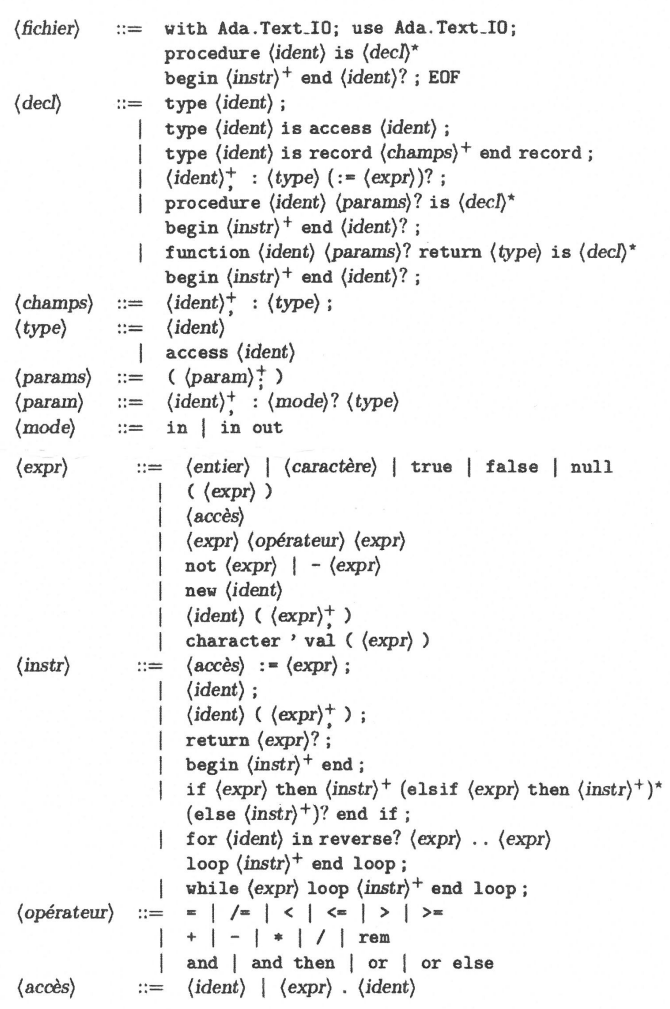
\includegraphics[width=0.8\textwidth]{grammaire_init}
        \caption{Grammaire initiale du Sujet}
    \end{figure}

    \subsection{Étapes de Transformation de la Grammaire}

    \subsection{Grammaire Originale en BNF}

    La grammaire initiale du langage "canAda", avant sa transformation en grammaire LL(1), se présente comme suit en BNF sans les regex:

    \begin{verbatim}
        fichier -> with Ada.Text_IO ; use Ada.Text_IO ;
                   procedure ident is <decls> begin <instrs> end <hasident> ; EOF

        decl -> type ident ;
               | type ident is access ident ;
               | type ident is record <champs> end record ;
               | <identsep> : <type> <typexpr> ;
               | procedure ident <hasparams> is <decls> begin <instrs> end <hasident> ;
               | function ident <hasparams> return <type> is <decls> begin <instrs> end <hasident> ;

        decls -> <decl> <decls>
                | ε

        hasident -> ident
                   | ε

        identsep -> ident , <identsep>
                   | ident

        champ -> <identsep> : <type> ;

        champs -> <champ> <champs>
                 | <champ>

        type -> ident
               | access ident

        params -> ( <paramsep> )

        hasparams -> <params>
                    | ε

        paramsep -> <param> ; <paramsep>
                   | <param>

        typexpr -> := <expr>
                  | ε

        param -> <identsep> : <mode> <type>

        mode -> in
               | in out
               | ε

        expr -> entier
               | caractère
               | true
               | false
               | null
               | ( <expr> )
               | <accès>
               | <expr> <opérateur> <expr>
               | not <expr>
               | - <expr>
               | new ident
               | ident ( <exprsep> )
               | character ' val ( <expr> )

        exprsep -> <expr> , <exprsep>
                  | <expr>

        hasexpr -> <expr>
                  | ε

        instr -> <accès> := <expr> ;
                 | ident ;
                 | ident ( <exprsep> ) ;
                 | return <hasexpr> ;
                 | begin <instrs> end ;
                 | if <expr> then <instrs> <elsif> <else> end if ;
                 | for ident in <hasreverse> <expr> .. <expr> loop <instrs> end loop ;
                 | while <expr> loop <instrs> end loop ;

        elsif -> elsif <expr> then <instrs> <elsif>
                 | ε

        else -> else <instrs>
                 | ε

        hasreverse -> reverse
                      | ε

        instrs -> <instr> <instrs>
                  | <instr>

        opérateur -> = | /= | < | <= | > | >= | + | - | * | / | rem | and | and then | or | or else

        accès -> ident
                | <expr> . ident

    \end{verbatim}

    \subsubsection{Élimination de la Récursivité à Gauche}
    La grammaire initiale comportait plusieurs instances de récursivité à gauche. Par exemple, la règle:
    \begin{verbatim}
        expr -> <accès>
        accès -> ident | <expr> . ident
    \end{verbatim}
    a été transformée en:
    \begin{verbatim}
        expr -> ident primary2
        primary2 -> ( exprsep ) acces | acces
        acces -> . ident acces | ε
    \end{verbatim}
    Cette modification élimine la (double ici) récursivité à gauche, rendant la grammaire adaptée pour une analyse LL(1).
    Une autre récursivité à gauche a été supprimé mais elle a été faite aussi à travers la priorisation des règles.

    \subsubsection{Factorisation à Gauche}
    La factorisation à gauche a été nécessaire pour certaines règles. Par exemple:
    \begin{verbatim}
        exprsep -> <expr> , <exprsep>
        exprsep -> <expr>
    \end{verbatim}
    a été réécrite en:
    \begin{verbatim}
        exprsep -> <expr> exprsep'
        exprsep' -> , <expr> exprsep' | ε
    \end{verbatim}
    Ceci assure que la règle peut être analysée de manière déterministe en LL(1).

    \subsubsection{Gestion des Priorités de Calculs}
    Pour gérer correctement les priorités des opérations, la grammaire a été ajustée. Par exemple, les opérations de multiplication et division ont été séparées des opérations d'addition et de soustraction pour respecter leur priorité:
    \begin{verbatim}
        expr -> <expr> <opérateur> <expr>
    \end{verbatim}
    a été réécrite en:
    \begin{verbatim}
        expr -> or_expr
        or_expr -> and_expr or_expr'
        or_expr' -> or or_expr'2 | ε
        or_expr'2 -> and_expr or_expr'
        or_expr'2 -> else and_expr or_expr'
        and_expr -> not_expr and_expr'
        \end{verbatim}
    [\dots]
    \begin{verbatim}
        unary_expr -> - unary_expr
        unary_expr -> primary
        primary -> entier
        primary -> caractère
        primary -> true
        primary -> false
        primary -> null
        primary -> ( expr )
        primary -> ident primary2
        primary -> new ident
        primary -> character ' val ( expr )
    \end{verbatim}
    Cela permet de respecter la hiérarchie des opérations dans les expressions arithmétiques.

    Les ensembles de sélection distincts ont été calculés pour assurer une sélection univoque lors de l'analyse.

    Ces étapes illustrent comment la grammaire initiale a été transformée en une grammaire LL(1), adaptée pour une analyse syntaxique efficace et précise du langage "canAda".

    \subsection{Grammaire Transformée en LL(1)}
    La grammaire transformée en LL(1) se présente comme suit:
    \begin{verbatim}
        fichier -> withAda.Text_IO;useAda.Text_IO; procedure ident is decls begin instrs end hasident ; EOF
        decl -> type ident hasischoose ;
        decl -> identsep : type_n typexpr ;
        decl -> procedure ident hasparams is decls begin instrs end hasident ;
        decl -> function ident hasparams return type_n is decls begin instrs end hasident ;

        hasischoose -> is accorrec | ε

        accorrec -> access ident
        accorrec -> record champs end record

        decls -> decl decls
        decls -> ε

        hasident -> ident
        hasident -> ε

        identsep -> ident identsep2

        identsep2 -> , identsep
        identsep2 -> ε

        champ -> identsep : type_n ;

        champs -> champ champs2

        champs2 -> champs | ε

        type_n -> ident
        type_n -> access ident

        params -> ( paramsep )

        hasparams -> params
        hasparams -> ε

        paramsep -> param paramsep2

        paramsep2 -> ; paramsep
        paramsep2 -> ε

        typexpr -> := expr
        typexpr -> ε

        param -> identsep : mode type_n

        mode -> in modeout
        mode -> ε

        modeout -> out
        modeout -> ε

        expr -> or_expr

        or_expr -> and_expr or_expr'

        or_expr' -> or or_expr'2
        or_expr' -> ε

        or_expr'2 -> and_expr or_expr'
        or_expr'2 -> else and_expr or_expr'

        and_expr -> not_expr and_expr'

        and_expr' -> and and_expr'2
        and_expr' -> ε

        and_expr'2 -> not_expr and_expr'
        and_expr'2 -> then not_expr and_expr'

        not_expr -> equality_expr not_expr'

        not_expr' -> not equality_expr not_expr'
        not_expr' -> ε

        equality_expr -> relational_expr equality_expr'

        equality_expr' -> = relational_expr equality_expr'
        equality_expr' -> /= relational_expr equality_expr'
        equality_expr' -> ε

        relational_expr -> additive_expr relational_expr'

        relational_expr' -> < additive_expr relational_expr'
        relational_expr' -> <= additive_expr relational_expr'
        relational_expr' -> > additive_expr relational_expr'
        relational_expr' -> >= additive_expr relational_expr'
        relational_expr' -> ε

        additive_expr -> multiplicative_expr additive_expr'

        additive_expr' -> + multiplicative_expr additive_expr'
        additive_expr' -> - multiplicative_expr additive_expr'
        additive_expr' -> ε

        multiplicative_expr -> unary_expr multiplicative_expr'

        multiplicative_expr' -> * unary_expr multiplicative_expr'
        multiplicative_expr' -> / unary_expr multiplicative_expr'
        multiplicative_expr' -> rem unary_expr multiplicative_expr'
        multiplicative_expr' -> ε

        unary_expr -> - unary_expr
        unary_expr -> primary

        primary -> entier
        primary -> caractère
        primary -> true
        primary -> false
        primary -> null
        primary -> ( expr )
        primary -> ident primary2
        primary -> new ident
        primary -> character ' val ( expr )

        primary2 -> ( exprsep ) acces
        primary2 -> acces

        exprsep -> expr exprsep2

        exprsep2 -> , exprsep
        exprsep2 -> ε

        hasexpr -> expr
        hasexpr -> ε

        instr -> ident instr2
        instr -> return hasexpr ;
        instr -> begin instrs end ;
        instr -> if expr then instrs elifn elsen end if ;
        instr -> for ident in hasreverse expr .. expr loop instrs end loop ;
        instr -> while expr loop instrs end loop ;

        instr2 -> instr3 := expr ;
        instr2 -> ( exprsep ) instr3 hasassign ;
        instr2 -> ;

        instr3 -> . ident instr3
        instr3 -> ε

        hasassign -> := expr
        hasassign -> ε

        elifn -> elif expr then instrs elifn
        elifn -> ε

        elsen -> else instrs
        elsen -> ε

        hasreverse -> reverse
        hasreverse -> ε

        instrs -> instr instrs2

        instrs2 -> instr instrs2
        instrs2 -> ε

        acces -> . ident acces
        acces -> ε
    \end{verbatim}

    \subsection{Table LL(1)}\label{subsec:table-ll(1)}

    \begin{figure}[H]
        \centering
        
\includegraphics[width=0.8,angle=90]{tableau_parsing}
        \caption{Table LL(1)}
    \end{figure}

    \section{Analyse Lexicale pour canAda}

    L'analyse lexicale, une étape cruciale dans le processus de compilation, est gérée par notre classe `Lexer`. Cette classe est responsable de la conversion du code source en une série de tokens, facilitant ainsi l'analyse syntaxique ultérieure.

    \subsection{Structure et Fonctionnement du Lexer}

    La classe `Lexer` lit le code source et identifie les différents tokens en se basant sur un ensemble de règles prédéfinies. Chaque token est une instance de la classe `Token`, qui contient des informations telles que le type de token et la valeur lexicale associée.

    \subsection{Gestion des Tokens}

    Des classes spécifiques, comme `Tag` et `PeekingReader`, sont utilisées pour catégoriser les tokens et gérer efficacement la lecture en avance du code source. La classe `Tag` définit les différents types de tokens, tandis que `PeekingReader` permet de lire en avance dans le flux de caractères pour identifier correctement les tokens complexes.

    \subsection{Optimisation et Fiabilité}

    Le `Lexer` est conçu pour être à la fois rapide et fiable, capable d'identifier précisément les tokens même dans des cas de syntaxe complexe. Cette précision est essentielle pour garantir une analyse syntaxique sans erreur dans les étapes suivantes du processus de compilation.

    \section{Analyse Syntaxique}

    La classe `Parser` a été conçue pour analyser les programmes écrits dans le langage "canAda". Chaque méthode de cette classe correspond à un non-terminal de la grammaire LL(1) et est responsable de l'analyse d'une structure syntaxique spécifique du langage.

    \subsection{Structure et Fonctionnement}

    Dans notre `Parser`, chaque fonction représente un non-terminal de la grammaire. Par exemple, une méthode `expr()` est utilisée pour analyser les expressions, correspondant au non-terminal `expr` de la grammaire. Ces méthodes sont appelées récursivement pour construire l'arbre syntaxique du programme source.

    \subsection{Interaction avec l'Analyseur Lexical}

    Le `Parser` interagit étroitement avec l'analyseur lexical, recevant un flux de tokens qui sont analysés selon les règles de la grammaire. Cette interaction est cruciale pour la décomposition correcte du programme source en ses composants syntaxiques.

    \subsection{Gestion des Erreurs Syntaxiques}

    Un aspect essentiel du `Parser` est sa capacité à gérer les erreurs syntaxiques. Lorsque le programme source ne respecte pas les règles de la grammaire, des messages d'erreur descriptifs sont générés, facilitant la localisation et la correction des erreurs par les développeurs. On a notamment appliqué le "panic mode" pour gérer les erreurs syntaxiques. Le Parser continue à analyser le programme source jusqu'à la fin tout en indiquant les erreurs rencontrées.

    \section{Construction de l'Arbre Abstrait Syntaxique pour canAda}

    La construction de l'arbre abstrait syntaxique (AST) est une étape essentielle du processus de compilation du langage "canAda". L'AST représente la structure syntaxique du programme source d'une manière qui est à la fois concise et facile à manipuler pour les étapes suivantes de la compilation.

    \subsection{Structure et Fonctionnement de l'AST}

    Notre système d'AST est construit autour de la classe `ASTNode`, qui sert de classe de base pour les différents types de nœuds de l'arbre. Chaque nœud spécifique, comme `OperatorNode`, `ParameterNode`, ou `ProgramNode`, hérite de `ASTNode` et représente une construction syntaxique spécifique du langage.

    \subsection{Représentation des Structures Syntaxiques}

    Les nœuds de l'AST capturent les éléments essentiels des structures syntaxiques du programme, comme les opérations, les paramètres, et la structure globale du programme. Par exemple, `OperatorNode` représente une opération arithmétique ou logique, tandis que `ProgramNode` représente la structure globale du programme canAda.

    \subsection{Rôle dans le Processus de Compilation}

    L'AST joue un rôle central dans le processus de compilation. Après l'analyse syntaxique, le programme source est transformé en un AST, qui est ensuite utilisé pour les étapes de vérification sémantique, d'optimisation, et de génération de code. Cette représentation permet une manipulation plus aisée et plus efficace du programme source.

    \section{Tests et Validation}

    \section{Gestion de projet}
    \subsection{Équipe de projet}
    Ce projet est un projet local réalisé en groupe de 4 personnes~:
    \begin{itemize}
        \item Alexis MARCEL
        \item Lucas LAURENT
        \item Noé STEINER
        \item Mathias AURAND-AUGIER
    \end{itemize}
    Le comité de pilotage est constitué de~:
    \begin{itemize}
        \item Anne-Claire HEURTEL
        \item Olivier FESTOR
        \item Gérald OSTER
    \end{itemize}
    Ces personnes constituent les parties prenantes de notre projet ainsi que les acteurs influents sur le livrables.

    \subsection{Organisation au sein de l’équipe projet}
    Nous avons réalisé plusieurs réunions, en présentiel dans les locaux de Télécom Nancy mais la plupart de notre collaboration a eu lieu sur Discord. Ces réunions nous ont permis de mettre en commun nos avancées régulièrement, de partager nos connaissances sur des problématiques et de nous organiser de manière optimale.
    En plus des réunions d'avancement régulières, nous avons également réalisé des réunions techniques afin de résoudre un problème ou bien de réfléchir à la conception.
    Les comptes rendus des réunions réalisées sont présents dans l’\hyperlink{annexe1}{Annexe 1}.

    Contrairement au premier projet, nous avons choisi de travailler cette fois-ci tous ensemble plutôt qu'individuellement. Nous avons donc utilisé une
    application pour que nous puissions tous modifier le code en même temps, ce qui nous a permis de tous travailler sur le même code en même temps.

    Ensuite, nous avons utilisé GitLab pour gérer les différentes versions du développement de notre application, ainsi que les différentes
    branches nous permettant de travailler simultanément sans conflit.

    Enfin, la rédaction des differents comptes rendus de réunion et des rapports ont été rédigé en \LaTeX.

    \subsection{Objectifs SMART}
    La méthode SMART que l'on rappelle ci-dessous nous a permis de définir nos différents objectifs :

    \subsection{Matrice des objectifs}
    Nous avons conçu, à l'aide de la méthode SMART, la matrice des objectifs suivante :

    En ce qui concerne, le livrable, il sera difficile, compte tenu des délais d'attendre tous les objectifs du projet.
    \subsection{Triangle qualité-cout-délai}
    Afin d’établir des objectifs cohérents, et réalisables dans les délais, nous avons réalisé le triangle qualité-coût-délai. On remarque ainsi, les délais étant courts, que nous avons tout intérêt à ne pas se fixer des objectifs trop ambitieux sous peine de devoir renoncer à certaines fonctionnalités et de ne pas rendre le livrable annoncé initialement.


    \subsection{Matrice SWOT}
    Afin d’avoir une vision plus globale de nos ressources et des facteurs internes et externes agissant sur le projet, nous avons ensuite réalisé la matrice SWOT (Strengths, Weaknesses, Opportunities, Threats) de notre projet.


    On peut ainsi remarquer que notre projet présente de nombreux points forts notamment grâce aux connaissances acquises lors des cours de Télécom Nancy
    mais également de par l’expérience forte de deux des membres de l’équipe projet.  Cependant, plusieurs facteurs internes constituent nos faiblesses
    notamment les courts délais qui nous obligent à être concis et efficaces dans notre travail. Cependant, nous avons également des opportunités notamment
    celle de pouvoir demander de l'aide aux autres élèves et aux professeurs, ou encore le fait que les salles soient ouvertes et à notre disposition pour
    les réunions de groupe.

    De plus, nous devons anticiper les charges de travail dans le cadre de notre formation à Télécom Nancy qui s'avèrent être plus élevées au mois de mai
    pour les partiels de fin d'année. Nous allons donc devoir prendre cela en compte dans notre gestion des tâches.

    \subsection{Profil de projet}

    Afin d’avoir une vision plus globale sur notre projet, nous avons également réalisé le profil du projet (le budget étant égal à 0, nous avons choisi de ne pas le représenter dans notre profil). On remarque que, du fait des nombreuses fonctionnalités que nous avons l’intention d’implémenter dans notre application, que notre projet est de taille moyenne mais de complexité élevée.

    Cependant, les enjeux du projet ne sont pas très importants (en dehors de la note finale qui compte dans notre moyenne) car l'échec du projet n'engendrera pas la chute d'une organisation et le budget est négligeable.

    De plus, au vu de l’état de l’art établi, l’innovation du projet est importante puisque peu d'application de ce type existent actuellement.



    \subsection{WBS~: comment concrétiser l’application}
    Ceci étant fait, nous avons maintenant choisi de détailler les lots de travail à effectuer pour fabriquer notre application. Nous avons ainsi réalisé le WBS (Work Breakdown Structure) de notre application~: il apparait ainsi les grandes étapes de notre projet que sont~: définition du cadre de l’application, développement des fonctionnalités de l’application et écriture du rapport.


    \subsection{Diagramme de Gantt~: planification}
    Maintenant que nous avons un détail des lots de travail qui constituent notre application, il faut maintenant les mettre en relation pour créer un planning efficace où chaque tâche est effectuée dans l’ordre.

    Ce diagramme est une première version générale des tâches à effectuer, il sera modifié et détaillé davantage une fois la conception et les maquettes du projet réalisées.

    \subsection{Matrice RACI}
    Nous avons choisi de ne pas faire de matrice RACI à cause des choix d'organisation que nous avons faits. En effet,
    nous avons décidé de travailler en groupe sur toutes les tâches, ce qui fait que nous sommes tous responsables de toutes les tâches et qu'il n'y a, de ce fait,
    pas de répartition précise des tâches.

    \subsection{Gestion des risques}
    Nous avons également pensé à prévoir une partie des risques pouvant se dresser sur notre route, les risques les plus classiques étant
    la gestion du temps et le manque de compréhension de certaines personnes de l'équipe.


    \section{Conclusion}

    En conclusion, ce projet s'est révélé être une expérience d'apprentissage extrêmement précieuse, nous permettant d'affiner et de développer nos compétences en programmation en langage C. Nous avons approfondi notre compréhension des structures de données, notamment comment les utiliser efficacement pour manipuler, stocker et accéder aux informations. Ce projet nous a aussi donné l'opportunité d'appliquer des algorithmes complexes, comme celui de Dijkstra, dans un contexte réel, nous permettant d'apprécier l'importance de ces outils dans la résolution de problèmes concrets.
    \newline
    En travaillant sur un problème réel - l'optimisation du placement des stations de charge pour véhicules électriques - nous avons pu saisir l'importance des implications de notre travail. Cela a ajouté une dimension plus large à notre apprentissage, en nous faisant comprendre comment les compétences techniques que nous avons acquises peuvent avoir un impact sur des questions d'une grande pertinence sociétale, comme la transition vers une mobilité plus durable.
    \newline
    De plus, la mise en évidence des enjeux de l'énergie durable dans notre projet nous a permis de nous immerger dans un secteur d'une importance cruciale pour l'avenir de notre société. L'efficacité de la distribution de l'énergie, en particulier pour les véhicules électriques, est une question clé dans la lutte contre les changements climatiques. En participant à la résolution de ce problème à travers notre projet, nous avons non seulement appliqué nos compétences techniques, mais également contribué à un domaine qui aura un impact durable et positif sur notre avenir.
    \newline
    En somme, ce projet nous a offert une occasion inestimable de croissance personnelle et professionnelle. Il nous a permis d'acquérir et de consolider des compétences techniques, tout en nous faisant prendre conscience de l'importance des implications de notre travail dans le monde réel, en particulier dans le domaine de la mobilité et de l'énergie durables.

    \section{Annexes}

\end{document}
